\section{Vinculación}

\subsection{Creación de vínculos}

La vinculación de usuarios (relativa al 
\nameref{sec:cu:vinculacion}) es una función que requiere la participación activa de \textbf{dos actores}, un Paciente y un Cuidador. El proceso paralelo puede verse en la \fref{dia:actividad_vinculacion}, mientras que la secuencia pormenorizada de los procesos y comunicaciones entre componentes se muestra en la \fref{dia:secuencia_vinculacion}.

Este proceso se puede comprender como tres subprocesos: la generación del \gls{token} o código de vinculación, el escaneo de este y la validación del vínculo. El primero de ellos es el realizado por el Paciente al elegir la opción de \textbf{Añadir vínculo} en su pantalla de vínculos. Al hacerlo, su aplicación móvil emitirá una petición de \gls{token} al respectivo \gls{endpoint} (\fref{api:generar_token_vinculacion}) de la \acrshort{api}, que lo generará en base a los datos de dicho paciente y lo enviará como respuesta. Una vez que la aplicación móvil lo reciba, lo convertirá en un \textbf{código QR} y lo mostrará en la pantalla del Paciente. Estos códigos tendrá un tiempo de caducidad que también se enviará junto al código, si llega a caducar, la aplicación solicitará otro código y lo mostrará en la pantalla.

\begin{figure}[H]
    \centering
    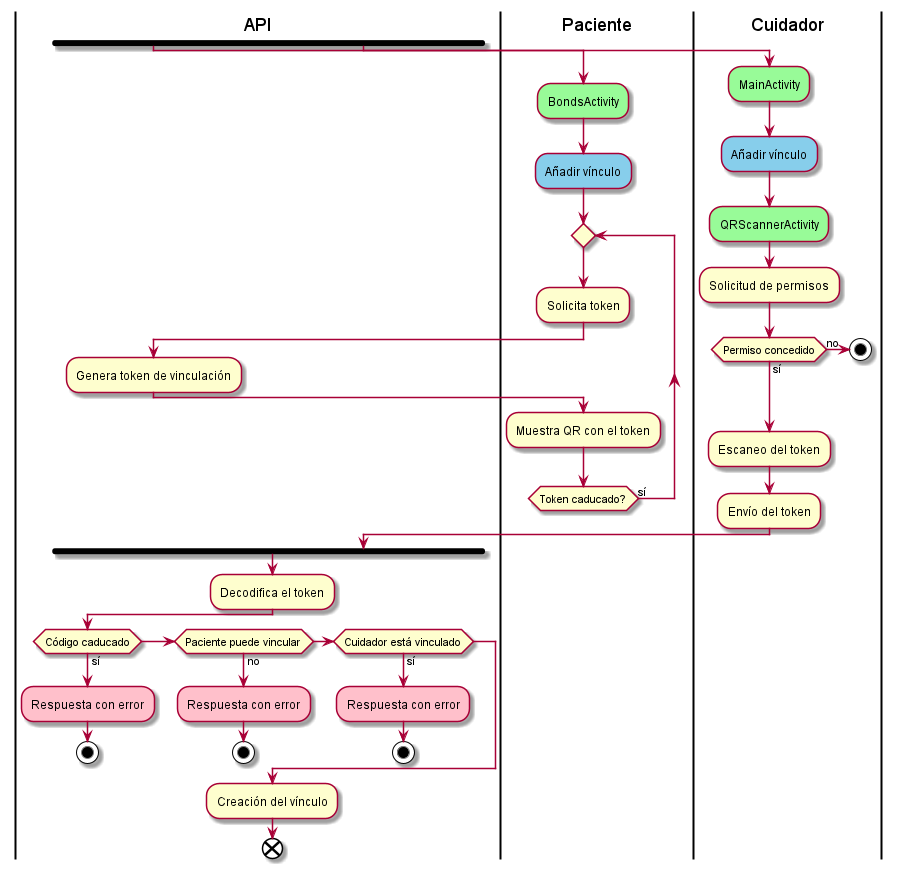
\includegraphics[width=0.7\textwidth]{images/Diseño/ActividadesVinculacion.png}
    \caption{Diagrama de actividades de la vinculación de usuarios}
    \label{dia:actividad_vinculacion}
\end{figure}

El Cuidador también iniciará su proceso por medio de una opción de \textbf{Añadir vínculo} situado en su pantalla principal. Al usarla la aplicación se dirigirá a la actividad del escáner y, previa obtención de requisitos de usuario, desde ella podrá enfocar el código QR mostrada en la aplicación del Paciente. La aplicación del Cuidador escaneará e \textbf{interpretará el código QR} obteniendo el \gls{token} que enviará a la \acrshort{api} con una petición al \gls{endpoint} del \fref{api:establecer_vinculo}.

\begin{figure}[H]
    \centering
    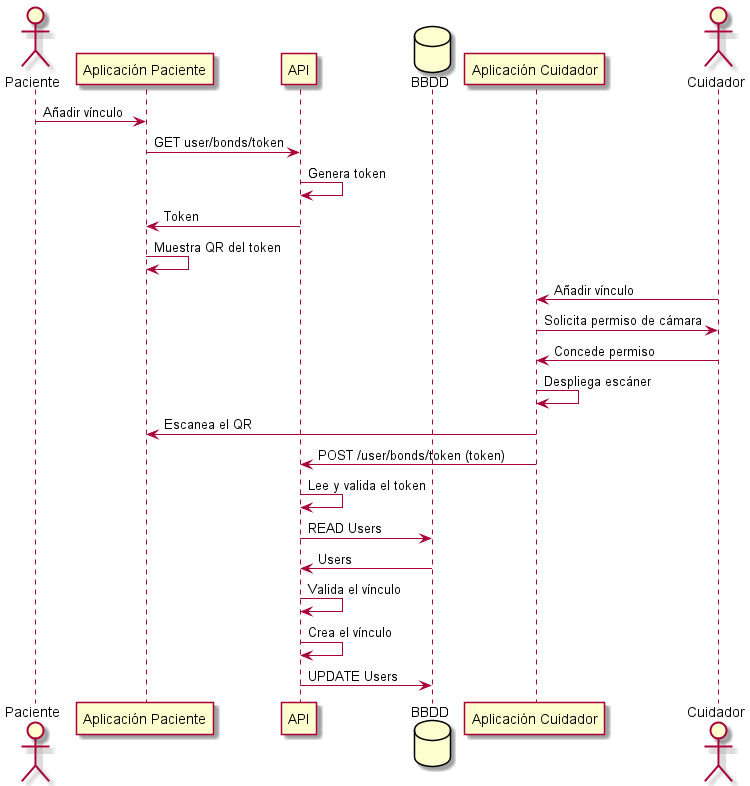
\includegraphics[width=0.5\textwidth]{images/Diseño/SecuenciaVinculacion.png}
    \caption{Diagrama de secuencia de la vinculación de usuarios}
    \label{dia:secuencia_vinculacion}
\end{figure}

Finalmente, una vez la \acrshort{api} reciba el \gls{token} del paciente comenzará su \textbf{lectura y validación}. Comprobará que el \gls{token} aún no haya caducado, si es el caso, lo leerá y obtendrá de él la ID del Paciente a vincular. Después solicitará la información de los usuarios para \textbf{comprobar si el vínculo es posible}. Si ese Paciente aún puede vincular más Cuidadores y el Cuidador no está vinculado, entonces la \acrshort{api} creará el vínculo añadiendo a cada uno de los actores a la lista de vínculos del otro, tras lo que actualizará los datos de ambos en la base de datos. De esta forma \textbf{el vínculo se habrá creado}.
